\chapter{Introduction}

Provide a general introduction to the area for the degree project. Use references!

Link things together with references. This is a reference to a section: \ref{sec:background}.

\section{Background}
\label{sec:background}
Quadruped robots have the potential to work in unstructured, severe and dangerous environments\cite{mengReviewQuadrupedRobots2016}, some specific examples of how quadruped robots could be used include search and rescue missions\cite{hawkesSoftRobotThat2017}, moving items on industrial production lines\cite{gehringANYmalFieldSolving2021} and scientific research\cite{hewingLearningbasedModelPredictive2020}. In comparison to  rigid legs, which can be modeled using multi-body dynamics for their dynamic movements, soft legs with soft actuators are more challenging to be modeled and controlled than rigid legs due to their non-linearity\cite{slotineAppliedNonlinearControl1991} and time variant properties\cite{wangControlStrategiesSoft2022}, such as hysteresis and drift, where the high non-linearity of soft materials makes them difficult to predict and control, and the hysteresis and drift can also increase the occurrence of unpredictable behaviors. Furthermore, the need to consider continuum mechanics, which deals with the behavior of continuously deformable materials with infinite \ac{DoF}\cite{polygerinosSoftRoboticsReview2017}, adds an extra level of complexity. 

In general, the control to a soft robot still require further research to establish the internal connection with control science\cite{wangControlStrategiesSoft2022}. Typically, the loads of rigid legs are different between the two cases of leg suspension and stepping on the ground\cite{biswalDevelopmentQuadrupedWalking2021}, which means that the dynamics of the quadruped robot is a mixture of continuous and discrete, such that the model is continuous when touching the ground or when hovering, but there is a sudden change from hovering to touching the ground, which makes the model behave a discrete. In addition, because of the influence of external gravity, the force required to move the motor at the same angle is different for different leg suspension positions, so the leg model of the quadruped is nonlinear, so that it is common to use a model predictive controller for rigid quadruped robots. However, it is not easy to predict the behavior of a soft robot if using a model predictive controller\cite{BemporadLinearTimevaryingNonlinearMPC}, so it is desired to have more identical solutions for the controllers, whereby the  reinforcement learning came to our mind\cite{hewingLearningbasedModelPredictive2020}. 

As the complexity of robotics increases, \ac{RL} is increasingly required to develop robust control algorithms with high \ac{DoF}s and time variant properties\cite{zhangEffectiveSoftRobot2017}. The rapid development of AI provides an alternative solution to take into account the nonlinear properties of novel materials and soft robots\cite{tangModelbasedOnlineLearning2021}. \ac{MFRL} is a type of reinforcement learning where an agent learns to make decisions based on experiences and rewards obtained from the environment, without having an explicit model of the environment. The agent directly can map observations to actions, through trial and error, without considering the underlying dynamics of the environment\cite{arulkumaranDeepReinforcementLearning2017}. The goal of model-free reinforcement learning is to learn a policy $\Pi$, which is a mapping from states to actions, that maximizes the expected cumulative reward over time. The \ac{MBRL} refers to a type of \ac{RL} where an agent learns optimal behavior by learning a model of the environment by taking actions and observing the outcomes that include the next step and the immediate reward\cite{rayModelBasedReinforcementLearning2010}. 
\begin{figure}[hp]
    \centering
    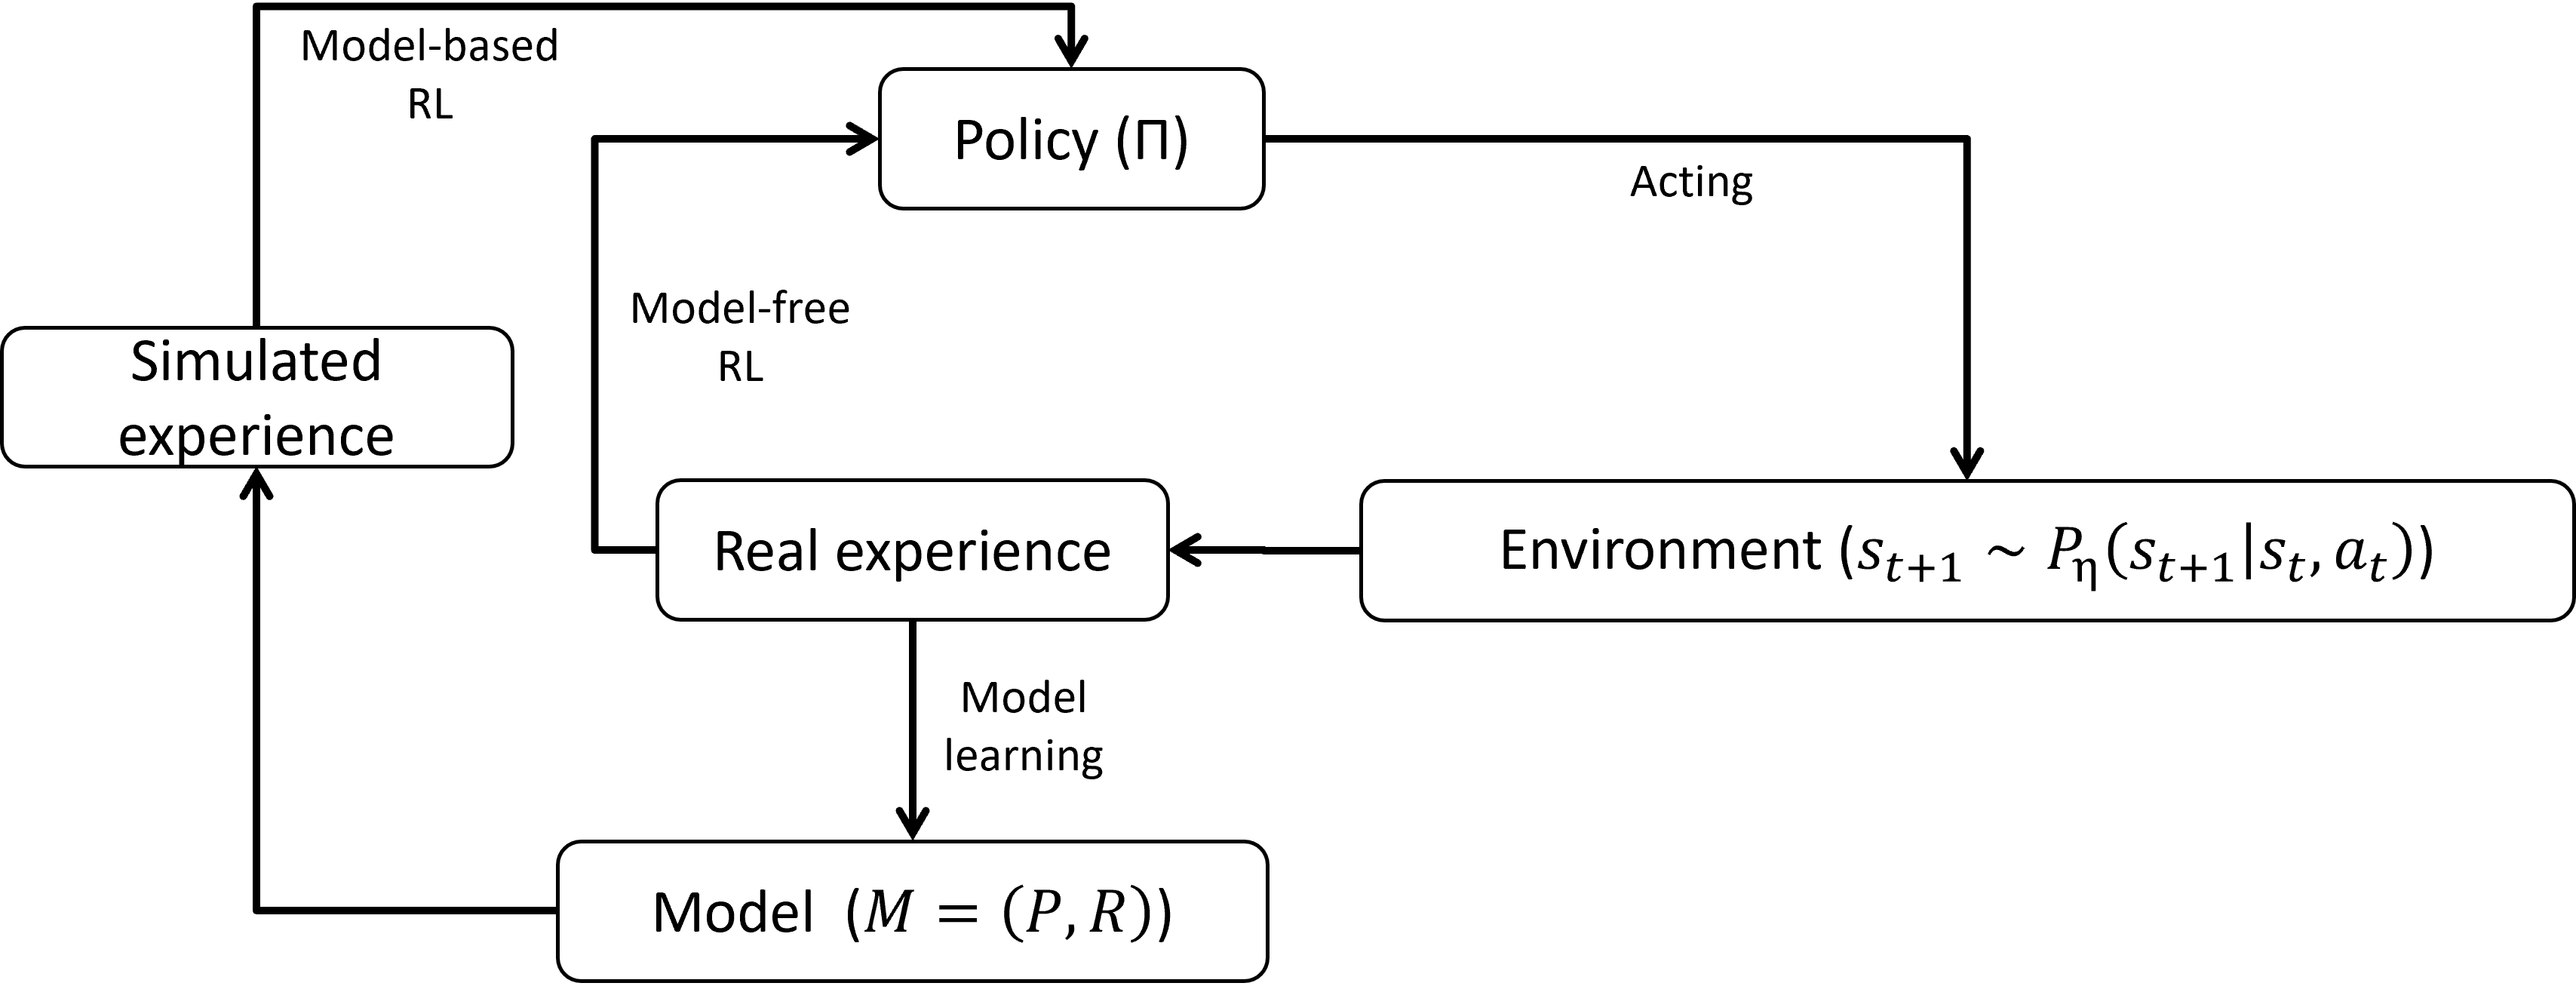
\includegraphics[width=\textwidth]{figures/model.png}
    \caption{Model-free \ac{RL} vs. Model-based \ac{RL}}
    \label{fig:demo}
\end{figure}

Typically, the model can be considered as a combination of state transition distribution $P_\eta$ and reward function $R_\eta$, $$M = (P,R) \textrm{ where } s_{t+1}\sim P_\eta(s_{t+1}|s_t, a_t) \textrm{ and } r_{t+1}\sim R_\eta(r_{t+1}|s_t, a_t)$$ $s_t$ is the state at time $t$, $r_t$ is the reward at time $t$ and $a_t$ is the action at time $t$. Model-based \ac{RL} learns an abstract model of the environment to plan the optimal policy. This model can be used to simulate the consequences of its actions, allowing it to make informed decisions, which makes it applicable to handle more complex environments, as it can make use of a model of the environment's dynamics. Therefore, model-based \ac{RL} requires a prior knowledge of the domainology\cite{tangModelbasedOnlineLearning2021}, as a model needs to be created and maintained. The domain of the model-based \ac{RL} refers to the context or environment in which the \ac{RL} agent is operating, which determines the available actions, observations, and rewards, and hence influences the behavior of the agent\cite{langExplorationRelationalDomains}. In model-based \ac{RL}, the agent needs to build a model of the dynamics of the system within the domain, and this model should accurately represent the true behavior of the system in order for the agent to learn effectively.

In the previous studies\cite{thorapallimuralidharanContinuumActuatorBased2020} completed by KTH Mechatronics and Embedded Control Systems Unit, tendon-driven soft continuum actuators were implemented on 3D/4D printed structures to operate as the legs of quadruped robots. Specifically, the tendons are used to transmit the force from motors, while the soft material acts as the core and the rigid disc acts as the tendon guide to form the actuator body. Since soft legs are inherently compliant to the terrain, they have had an increased capability of traversing complicated environments. Based on this soft leg, a soft quadrupedal robot prototype was developed, and the gait analysis were conducted to enable the robot to walk\cite{daneliaStructureGaitOptimizationof2021}. Modelling for the actuators and legs are quite important for closed loop control, since the robots will benefit from feedback to the closed loop control when interacting with the terrine. Therefore, the KTH team\cite{muralidharanSoftQuadrupedRobot2021} have already investigated the modeling process of a quadruped robot enabled by four tendon-driven continuum actuators on MATLAB Simulink. Based on the developed soft robot model, an optimal gait controller was developed by a model-free reinforcement learning approach\cite{jiSynthesizingOptimalGait2022} recently.
\section{Motivation}
 The gait controller was first trained and evaluated in the simulation platform, and then it is deployed in the physical robot prototype for experimental testing. The developed gait control can be optimum, but the achieved walking speed on the real robot was half of the target speed in the simulation\cite{jiSynthesizingOptimalGait2022}. The current approach also applies Simulink Multibody functions to describe the robot dynamics, which achieves a relatively accurate physical representation but at a very low time efficiency of the simulator. Thus, the learning efficiency of the \ac{RL} algorithm is limited, and it is desired to be improved. The concept of model-based reinforcement learning is considered to generate a functional representation of the robot’s interaction with the external environment, so as to resemble the physical plant model and provide the state update feedback with high accuracy efficiently\cite{rayModelBasedReinforcementLearning2010}. In model-based \ac{RL}, the agent learns a surrogate model of the environment, which can be used to make predictions about the future state of the environment and the possible outcomes of different actions, which allows the agent to plan ahead and make more informed decisions, allowing it to learn more efficiently and solve tasks more effectively\cite{polydorosSurveyModelBasedReinforcement2017}. Compared to the Simulink Multibody functions, this predictive model is expected to improve the simulation efficiency while guaranteeing the model fidelity, which can benefit the following \ac{RL} gait training. 
 
 Furthermore, the Simscape soft robot model was used as the environment model for the \ac{RL} agent\cite{jiSynthesizingOptimalGait2022}, which monitors the locomotion of soft quadruped robots. Model-based \ac{RL} is prior to model-free \ac{RL} in certain scenarios, some literature\cite{polydorosSurveyModelBasedReinforcement2017,wangBenchmarkingModelBasedReinforcement2019} stated that at robotic applications, the model-based \ac{RL} utilizes a model of the environment to make predictions about the outcomes of different actions, which can lead to more efficient learning. The model-free \ac{RL} learns directly from experience without building a model of the environment\cite{arulkumaranDeepReinforcementLearning2017}, and it often require large amounts of data to learn a policy that can achieve optimal performance\cite{calisirModelFreeReinforcementLearning2019}. With a surrogate model, a model-based \ac{RL} agent can simulate different possible future trajectories, allowing it to select actions that maximize rewards\cite{fazeliSeeFeelAct2019}. Model-based \ac{RL} approach can also help reduce the sample complexity and improve the data efficiency of the learning process\cite{atkesonComparisonDirectModelbased1997}. The policy learnt by the surrogate model is different from that by model-free \ac{RL}\cite{fazeliSeeFeelAct2019}, which might make a significant difference to the policy learnt and affect the walking performance of soft quadruped robots, so the evaluation of the controllers will not focus on the algorithms, but on the benefits to the ability of a robot to walk in terms of stability, walking speed and cost-of-transport.

 However, the input value to the \ac{RL} agent consists of state space and action space, and the state space was defined by available sensor measurements, including robot moving velocity in three directions, rotational angle in three directions and normalized contact force on four feet\cite{jiSynthesizingOptimalGait2022}. The action space was defined by motors on the legs, and three motors on each leg\cite{jiSynthesizingOptimalGait2022}. Therefore, the state-action space of the reaches 22 dimensions, which expands the computational requirements and leads to sparsity in the reward function. As discussed in the background, the state space of the surrogate model consists of state transitions states and reward function states, which will also reach a significant high dimensions. In order to increase the learning efficiency, there could be several ways to restrict the state space of the plant model, one of them could be restricting the state-action space in the model, for example, the feature extraction, which means some relevant features could be extracted and composed based on the kinematics of certain gaits. In the previous training\cite{jiSynthesizingOptimalGait2022}, the gait controllers were learnt from scratch, but rigid quadruped robots can have certain patterns of leg movements, including trot, pace, bound, pronk, gallop, etc.\cite{zhongAnalysisResearchQuadruped2019}, so that if the gait controllers could be defined on certain patterns, the gait controllers could be simplified by some certain gaits and some actions could be composed to reduce the state-action space so as to increase the learning efficiency\cite{owakiQuadrupedRobotExhibiting2017}. The trot is a common gait in all domestic quadrupeds\cite{jiOmnidirectionalWalkingQuadruped2022}. It is well-suited for rough, irregular ground and for traveling long distances at a fair rate of speed, because work is spread evenly over all four limbs, and diagonal support makes it easy to maintain equilibrium\cite{fletcherTrot2012}, so it is considered to restrict the pattern of a soft quadruped robot to trot. Another method to restrict the state space of the plant model is parameterization, the phases between gait generator and control policy could be studied and defined based on the abstraction of the quadruped robot to parameterize various gaits for robust control of rigid quadruped robots\cite{shaoLearningFreeGait2022}. Based on previous parameterization on the continuum actuators\cite{jiOmnidirectionalWalkingQuadruped2022}, such techniques could be considered to be applied on the surrogate model so as to increase the learning efficiency by reducing the search space of the state space.
\section{Research Questions} 
Due to the complexity of the state space of robot models, a limited amount of collected data may not provide a comprehensive understanding of the dynamics of the quadruped robot, which can result in decreased accuracy. The learning efficiency of current approaches to an optimal gait controller was low and expected to be improved. Thus, this project aims to explore and address these issues, and tries to solve them by model-based reinforcement learning. Therefore, the research questions come out as: 
\begin{enumerate}
    \item How to restrict the state space or design a surrogate model with high estimation accuracy of soft quadruped robots plant compared to using Simulink Multibody functions? This model could be extracted as a representation of the real system, allowing for efficient and accurate simulations and training. Some methods considered to restrict the state space:
    \begin{enumerate}
        \item Feature extraction, it involves selecting a subset of features based on the certain pattern of quadruped robots, i.e. trot.
        \item Parameterization, the higher-level abstractions of the state-action space, it will use phases between gait and real motors to parameterize gaits of quadruped robots.
    \end{enumerate}
    \item In comparison to model-free \ac{RL}, to what extend can the model-based \ac{RL} approach generate a better \ac{RL} agent and enhance the ability of a soft quadruped robot to walk in terms of stability, walking speed, and cost-of-transport? The enhancement than model-free \ac{RL} is a benchmark of this project. Furthermore, it is important to evaluate the performance of model-based \ac{RL}, and the evaluation of performance of this project focus on the simulation benefices, so what the trade-off is among the learning efficiency, the simulation accuracy and the long-term planning accuracy in order to train an optimal policy for gait control of soft quadruped robot?
\end{enumerate}

\section{Methods and Methodologies}
The main methods and methodologies applied towards answering the research questions are discussed in this section. The methodology includes four main parts: data collection and processing, model-based \ac{RL} algorithm development and comparison, evaluation and analysis, and validation.

\textbf{Model design}
\begin{enumerate}
    \item Extract the signals to motors from the typical trot of quadruped robots by studying the actuation of soft quadruped robot trot pattern.
    \item Obtain the model of soft quadruped robots and use it to generate simulation data using the Simscape model of the soft quadruped robot based on the extracted state space. 
    \item On the basis of proceeded data, design a surrogate model with high estimation accuracy of soft quadruped robot plant, which can effectively simulate the dynamics of the system and can be used to train an optimal policy for gait control. 
    % \item Preprocess the simulation data to reduce the dimensionality of the state space using the methods described in Research Question 1.
\end{enumerate}
\textbf{Model-based \ac{RL} algorithm development and comparison}
\begin{enumerate}
    \item Develop a model-based \ac{RL} algorithm for gait control of the soft quadruped robot using the extracted features and the reduced state space.
    \item Evaluate the algorithm's performance in simulation using metrics such as stability, walking speed, and cost-of-transport.
    \item Iterate on the algorithm's design and parameters to improve its performance.
    \item Evaluate and compare the previous model-free \ac{RL} algorithm's performance with the same metrics.
\end{enumerate}
\textbf{Evaluation and analysis}
\begin{enumerate}
    \item Evaluate the trade-offs between learning efficiency, simulation accuracy, and long-term planning accuracy in the context of training an optimal policy for gait control of the soft quadruped robot.
    \item Analyze the results and draw conclusions about the effectiveness of the proposed model-based \ac{RL} approach compared to model-free \ac{RL}.
\end{enumerate}
\textbf{Validation}
\begin{enumerate}
    \item Validate the proposed approach by implementing the optimal policy on the physical soft quadruped robot and measuring its performance in a real-world setting, measure the robot's performance in terms of walking speed, stability and cost-of-transport.
    \item Compare the physical robot's performance with the simulated results to validate the accuracy of the simulation and the effectiveness of the proposed approach.
\end{enumerate}

\section{Delimitations}
 This thesis will focus on exploring and addressing the issues of model-based reinforcement learning for optimal gait control of soft quadruped robots. For this particular study, there are several delimitations important to consider. Firstly, it focuses specifically on soft quadruped robots and does not take into account other types of robots or robotic systems. Secondly, simulations and experiments are limited to a controlled environment and may not accurately reflect real-world scenarios. Thirdly, the effects of external factors such as wind, terrain, or obstacles are not considered in this study. Additionally, the project assumes that the soft quadruped robot is functioning correctly and does not address potential hardware malfunctions or failures. Finally, this project is limited to a specific model-based  algorithm and does not consider other potential approaches or methods. It is important to note that these delimitations are not exhaustive and may vary depending on the specific research project. 
 
\section{Ethics and Sustainability}
The use of robotics and artificial intelligence raises ethical and sustainability considerations that need to be addressed in this project. One ethical consideration is related to the potential for the quadruped robot to be used for military or surveillance purposes, which could have negative impacts on privacy and human rights. To ensure that the robot is used ethically, the project will focus on the development of an optimal gait controller for soft quadruped robots for use in research and other non-military applications. Sustainability considerations include the environmental impact of the materials used in the construction of the robot, as well as the potential impact of the project on the environment through energy consumption and waste. To address these considerations, the project will use environmentally-friendly materials where possible and focus on energy efficiency in the design and testing of the robot.

Detailed description of these methodologies and methods should be presented in Chapter 3. In chapter 3, the focus could be research strategies, data collection, data analysis, and quality assurance.

Boxes can be used to organize content
\begin{tcolorbox}[title={Development environment for prototype}]
	\tt{
		\textbf{Operating systems }\\
		computer: Linux - kernel 4.18.5-arch1-1-ARCH\\
		android phone: 8.1.0\\
		~\\
		\textbf{Build tools}\\
		exp (build tool): version 55.0.4\\
		~\\
		...
	}
\end{tcolorbox}

\section{Outline}
In text, describe what is presented in Chapters 2 and forward. Exclude the first chapter and references as well as appendix. 
